\documentclass[a4paper]{scrreprt}
\usepackage[left=4cm,bottom=3cm,top=3cm,right=4cm,nohead,nofoot]{geometry}
\usepackage{import,graphicx,tabularx,listings,enumitem,subcaption}
\usepackage{xparse,multirow}
\usepackage{xcolor}
\usepackage{amsmath}
\setlength{\textfloatsep}{16pt}
\renewcommand{\labelenumi}{\alph{enumi})}
\renewcommand{\labelenumii}{\arabic{enumii}) }
\usepackage{float}

\usepackage{listings}
\usepackage{xcolor}

\lstset{
  basicstyle=\ttfamily\small,
  keywordstyle=\color{blue},
  commentstyle=\color{gray},
  stringstyle=\color{green!40!black},
  breaklines=true,
  frame=single,
  columns=fullflexible
}

% Base info for header
\newcommand{\baseinfo}[5]{
  \begin{center}
    \begin{tabular}{p{15cm}r}
      \vspace{-4.5pt}{ \Large \bfseries #1} & \multirow{2}{*}{} \\[0.4cm]
      #2 & \\[0.5cm]
    \end{tabular}
  \end{center}
  \vspace{-18pt}\hrule\vspace{6pt}
  \begin{tabular}{ll}
    \textbf{Names:} & #4\\
    \textbf{Group:} & #5\\
  \end{tabular}
  \vspace{4pt}\hrule\vspace{2pt}
  \footnotesize \textbf{Software Testing} \hfil - \hfil Summer 2024 \hfil - \hfil #3 \hfil - \hfil Sibylle Schupp / Daniel Rashedi \hfil \\
}

\lstdefinestyle{pythongrey}{
    language=Python,
    basicstyle=\ttfamily\small,
    keywordstyle=\color{blue},
    commentstyle=\color{gray},
    stringstyle=\color{green!50!black},
    backgroundcolor=\color{gray!10},
    showstringspaces=false,
    breaklines=true,
    frame=single,
    framesep=3pt,
    tabsize=4,
    numbers=left,
    numberstyle=\tiny\color{gray},
    numbersep=8pt,
    captionpos=b
}

% Question and answer environments
\newcounter{question}
\NewDocumentEnvironment{question}{m o}{%
  \addtocounter{question}{1}%
  \paragraph{\textcolor{red}{Task~\arabic{question}} - #1\hfill\IfNoValueTF{#2}{}{[#2]}}
  \leavevmode\\%
}{%
  \vskip 1em%
}

\NewDocumentEnvironment{aiTask}{}{
  \paragraph{\textcolor{red}{AI Review Task}}
  \leavevmode\\
}{
  \vskip 1em
}

\NewDocumentEnvironment{answer}{}{%
  \vspace{6pt}
  \leavevmode\\
  \textit{Answer:}\\[-0.25cm]
  {\color{red}\rule{\textwidth}{0.4mm}}
}{%
  \leavevmode\\
  {\color{red}\rule{\textwidth}{0.4mm}}
}

% ======= STUDENTS: START EDITING BELOW THIS LINE =======
\newcommand{\projectinfo}[4]{\baseinfo{Project - Submission Sheet}{#1}{#2}{#3}{#4}}
\newcommand{\name}{Maxim Zilke, Yossef Al Buni}
\newcommand{\group}{2}

\begin{document}
\projectinfo{Software Testing - Input Space Partitioning\small}{\today}{\name}{\group}

\addtocounter{question}{1}

%%%%%%%%%%%%%%%%
%%% Phase 02 %%%
%%%%%%%%%%%%%%%%

\begin{question}{Input Space Partitioning}
  \begin{enumerate}[topsep=0pt, leftmargin=*]
    \item Explain why the selected methods are suitable for the input domain model approach (1-2 sentences each)
          \begin{answer}
            \begin{lstlisting}[language=Python, caption={Maxim Zilke Function for parsing version strings}]
def _parse_version(version: str) -> tuple[int, int, int, int]:
    m = re.match(r"(\d+)\.(\d+)\.(\d+)(?:[+-](\d+))?", version)  # structure: MAJOR.MINOR.PATCH[+DISTANCE]
    if not m:
        raise ValueError(f"Invalid version string: '{version}'")

    major, minor, patch, distance = m.groups()
    return int(major), int(minor), int(patch), (0 if distance is None else int(distance))
\end{lstlisting}

The code is suitable for Input Space Partitioning because it breaks down the input values (version strings) into clearly defined parts (Major, Minor, Patch, and optional Distance), making it suitable to test different input values for each of the components[Maxim Zilke]

%%%%%%%%%%%%%%%%%%%%%%%%%%%%%%%%%%%%%%%%%%%%%%%%%%%%%%%%%%%%%%%%%%%%%%%%%%%%%%%%%%%
\begin{lstlisting}[language=Python, caption={Yossef Al Buni The funcrion searches for the suitable plugin based on a URL}]
def streams(self, url: str, options: Options | None = None, **params):
        _pluginname, pluginclass, resolved_url = self.resolve_url(url)
        plugin = pluginclass(self, resolved_url, options)
        return plugin.streams(**params)
\end{lstlisting}
This method processes user inputs (URLs) in various forms and forwards them to plugins that respond to supported streaming platforms. Since the behavior varies significantly depending on URL type, options, and additional parameters, the input space can be systematically partitioned – ideal for the application of Input Space Partitioning for efficient test coverage.

%%%%%%%%%%%%%%%%%%%%%%%%%%%%%%%%%%%%%%%%%%%%%%%%%%%%%%%%%%%%%%%%%%%%%%%%%%%%%%%%%%%

% other members

%%%%%%%%%%%%%%%%%%%%%%%%%%%%%%%%%%%%%%%%%%%%%%%%%%%%%%%%%%%%%%%%%%%%%%%%%%%%%%%%%%%

          \end{answer}

    \item Identify the input domain of your methods (2-3 sentences each)
          \begin{answer}
      

The input domain for the method \texttt{\_parse\_version} consists of all possible combinations of integers in the range from 0 to \texttt{MAX\_VALUE}. Letters and negative values are not allowed and will result in an error. The input must follow the format \texttt{X.Y.Z} or \texttt{X.Y.Z+N}, where \texttt{X}, \texttt{Y}, \texttt{Z}, and optionally \texttt{N} are integers [Maxim Zilke]. \\

%%%%%%%%%%%%%%%%%%%%%%%%%%%%%%%%%%%%%%%%%%%%%%%%%%%%%%%%%%%%%%%%%%%%%%%%%%%%%%%%%%%

 \textbf{Input Domain:} The input domain of the \texttt{streams()} method consists primarily of the \texttt{url} parameter, which can be any string representing a web address, and optionally an \texttt{options} object and additional keyword arguments (\texttt{**params}). Valid inputs include URLs supported by existing Streamlink plugins (e.g., Twitch, YouTube), while invalid inputs may include unsupported or malformed URLs. The method also accepts optional configurations that influence stream selection, making the domain a combination of structural URL validity, plugin support, and optional behavioral parameters. [Yossef Al Buni]

%%%%%%%%%%%%%%%%%%%%%%%%%%%%%%%%%%%%%%%%%%%%%%%%%%%%%%%%%%%%%%%%%%%%%%%%%%%%%%%%%%%

% other members

%%%%%%%%%%%%%%%%%%%%%%%%%%%%%%%%%%%%%%%%%%%%%%%%%%%%%%%%%%%%%%%%%%%%%%%%%%%%%%%%%%%
          \end{answer}

    \item Similar to Homework 02, gather the results of the following sub-tasks:
          \begin{enumerate}
            \item Identify reasonable characteristics of the possible input data
            \item Derive sets of equivalence classes from these characteristics (Note: At least one of your partitions must consist of a number of blocks $\geq 3$. Also make sure that you have enough characteristics and corresponding blocks to derive $12$ distinct tests from them later on.)
          \end{enumerate}
          \begin{answer}
          

%%%%%%%%%%%%%%%%%%%%%%%%%%%%%%%%%%%%%%%%%%%%%%%%%%%%%%%%%%%%%%%%%%%%%%%%%%%%%%%%%%%%%%%%%%%%%%%%%%%%%
            
\vspace{1em}
\centering
\small
\renewcommand{\arraystretch}{1.2}

\begin{tabular}{|p{2.5cm}|p{2.5cm}|p{2.5cm}|p{2.5cm}|p{2.5cm}|}
\hline
\textbf{Characteristic} & \textbf{Eq-Class 1} & \textbf{Eq-Class 2} & \textbf{Eq-Class 3} & \textbf{Eq-Class 4} \\
\hline
\texttt{q\textsubscript{1}}: sign of Major & \texttt{0} & \texttt{positive integer} & \texttt{negative integer} & \\
\hline
\texttt{q\textsubscript{2}}: sign of Minor & \texttt{0} & \texttt{positive integer} & \texttt{negative integer} & \\
\hline
\texttt{q\textsubscript{3}}: sign of Patch & \texttt{0} & \texttt{positive integer} & \texttt{negative integer} & \\
\hline
\texttt{q\textsubscript{4}}: sign of Distance & \texttt{0} & \texttt{positive integer} & \texttt{negative integer} & \\
\hline
\texttt{q\textsubscript{5}}: Format length & \texttt{length = 3 (X.Y.Z)} & \texttt{length = 4 (X.Y.Z+N)} & \texttt{length = 2 (missing parts)} & \\
\hline
\texttt{q\textsubscript{6}}: Characters & \texttt{all numeric} & \texttt{letters or symbols} & & \\
\hline
\texttt{q\textsubscript{7}}: Leading Zero & \texttt{no leading zero} & \texttt{leading zero} & \texttt{only zero} & \texttt{multiple zeros} \\
\hline
\end{tabular}
\vspace{0.5em}
\textbf{Table 1:} Input characteristics and equivalence classes for \texttt{\_parse\_version} by Maxim Zilke
%%%%%%%%%%%%%%%%%%%%%%%%%%%%%%%%%%%%%%%%%%%%%%%%%%%%%%%%%%%%%%%%%%%%%%%%%%%%%%%%%%%%%%%%%%%%%%%%%%%%%
    \begin{table}[H]
    \centering
    \small
    \renewcommand{\arraystretch}{1.2}
    \begin{tabular}{|p{2.5cm}|p{2.5cm}|p{2.5cm}|p{2.5cm}|p{2.5cm}|}
    \hline
    \textbf{Characteristic} & \textbf{Eq-Class 1} & \textbf{Eq-Class 2} & \textbf{Eq-Class 3} & \textbf{Eq-Class 4} \\
    \hline
    URL syntax & Well-formed & Malformed & Empty string & URL with leading/trailing spaces \\
    \hline
    Plugin availability & Supported plugin (e.g., Twitch) & Unsupported plugin (e.g., unknown.tv) & \textendash & \textendash \\
    \hline
    Options object & \texttt{None} & Valid \texttt{Options} with standard settings & Valid \texttt{Options} with special flags & \textendash \\
    \hline
    Additional parameters & No parameters & Valid parameter (e.g., stream types) & Invalid parameter key & Invalid parameter value \\
    \hline
    \end{tabular}
    \caption{Equivalence classes for the \texttt{streams()} method input domain}
    \label{tab:streams_method}
    \end{table}

%%%%%%%%%%%%%%%%%%%%%%%%%%%%%%%%%%%%%%%%%%%%%%%%%%%%%%%%%%%%%%%%%%%%%%%%%%%%%%%%%%%%%%%%%%%%%%%%%%%%%



          \end{answer}

    \item Can you identify any non-valid combinations of blocks from your characteristics? (1-2 sentences each)
          \begin{answer}
          %%%%%%%%%%%%%%%%%%%%%%%%%%%%%%%%%%%%%%%%%%%%%%%%%%%%%%%%%%%%%%%%%%%%%%%
          You can not have Distance = 0/ positive integer and length = X.Y.Z becasue if distance is active you have automaticaly length = X.Y.Z+N [Maxim Zilke]  \\
         %%%%%%%%%%%%%%%%%%%%%%%%%%%%%%%%%%%%%%%%%%%%%%%%%%%%%%%%%%%%%%%%%%%%%%%%

    Yossef: Yes, non-valid combinations can occur when a well-formed URL is combined with a nonexistent plugin (e.g., https://unknown.tv/stream) and invalid parameters, which would cause the plugin resolution or stream extraction to fail. Another invalid case is when a malformed or empty URL is paired with any valid plugin or options—since plugin resolution depends on a valid URL format, the rest of the inputs become irrelevant. [Yossef AL Buni] \\
          
        %%%%%%%%%%%%%%%%%%%%%%%%%%%%%%%%%%%%%%%%%%%%%%%%%%%%%%%%%%%%%%%%%%%%%%%%

        % other members

        %%%%%%%%%%%%%%%%%%%%%%%%%%%%%%%%%%%%%%%%%%%%%%%%%%%%%%%%%%%%%%%%%%%%%%%%
          \end{answer}
%%%%%%%%%%%%%%%%%%%%%%%%%%%%%%%%%%%%%%%%%%%%%%%%%%%%%%%%%%%%%%%%%%%%%%%%%%%%%%%%%%%%%%%%%%%%%%%%%%%%%
    \item Derive (at least) one representative value for each equivalence class. Which strategy did you use for the value selection?
          \begin{answer}
%%%%%%%%%%%%%%%%%%%%%%%%%%%%%%%%%%%%%%%%%%%%%%%%%%%%%%%%%%%%%%%%%%%%%%%%%%%%%%%%%%%%%%%%%%%%%%%%%%%%%
\textbf{strategy}: \\
The function is naturally divided into four parts, which are Major, Minor, Patch, and Distance. For each part, I selected 0 and all valid and invalid ranges. Furthermore i also added the characters as an invalid input. [Maxim Zilke]

\vspace{1em}
\centering
\small
\renewcommand{\arraystretch}{1.2}
\begin{tabular}{|p{2.5cm}|p{2.5cm}|p{2.5cm}|p{2.5cm}|p{2.5cm}|}
\hline
\textbf{Characteristic} & \textbf{Eq-Class 1} & \textbf{Eq-Class 2} & \textbf{Eq-Class 3} & \textbf{Eq-Class 4} \\
\hline

\texttt{q\textsubscript{1}}: sign of major Major & \texttt{0} & \texttt{from 1 to largest possible positive values} & \texttt{from -1 to largest possible negative value} & \texttt{}\\
\hline

\texttt{q\textsubscript{2}}: sign of Minor & \texttt{0} & \texttt{from 1 to largest possible positive values} & \texttt{from -1 to largest possible negative value}& \texttt{}\\
\hline

\texttt{q\textsubscript{3}}: sign of Patch & \texttt{0} & \texttt{from 1 to largest possible positive values} & \texttt{from -1 to largest possible negative value}& \texttt{} \\
\hline

\texttt{q\textsubscript{4}}: sign of Distance & \texttt{0} & \texttt{from 1 to largest possible positive values} & \texttt{from -1 to largest possible negative value} & \texttt{} \\
\hline

\texttt{q\textsubscript{5}}: Format length & \texttt{3 (X.Y.Z)} & \texttt{4 (X.Y.Z+N)} & \texttt{2 (X.Y)} & \texttt{}\\
\hline

\texttt{q\textsubscript{6}}: Characters& \texttt{40.23.40} & \texttt{a-z and all sonderzeichen} & \texttt{} & \texttt{}\\
\hline

\texttt{q\textsubscript{7}}: Leading Zero& \texttt{11.1.4} & \texttt{01.02.03} & \texttt{0.0.0.0} & \texttt{0.0.0+000}\\
\hline
\hline
\end{tabular}
\label{tab:parse-version-eqclasses}
\vspace{0.5em}
\noindent
\textbf{Table 1:} Input characteristics and equivalence classes for \texttt{\_parse\_version} by Maxim Zilke
%%%%%%%%%%%%%%%%%%%%%%%%%%%%%%%%%%%%%%%%%%%%%%%%%%%%%%%%%%%%%%%%%%%%%%%%%%%%%%%%%%%%%%%%%%%%%%%%%%%%%

\begin{table}[H]
\centering
\small
\renewcommand{\arraystretch}{1.2}
\begin{tabular}{|p{3.2cm}|p{3.5cm}|p{6cm}|}
\hline
\textbf{Characteristic} & \textbf{Equivalence Class} & \textbf{Representative Value} \\
\hline
URL syntax & Well-formed & \texttt{"https://twitch.tv/examplechannel"} \\
\cline{2-3}
           & Malformed & \texttt{"htp:/stream"} \\
\cline{2-3}
           & Empty string & \texttt{""} \\
\cline{2-3}
           & Leading/trailing spaces & \texttt{"  https://twitch.tv/examplechannel  "} \\
\hline
Plugin availability & Supported plugin & \texttt{"https://twitch.tv/examplechannel"} \\
\cline{2-3}
                    & Unsupported plugin & \texttt{"https://unknownplatform.com/live"} \\
\hline
Options object & \texttt{None} & \texttt{None} \\
\cline{2-3}
               & Valid standard options & \texttt{Options()} \\
\cline{2-3}
               & Valid special flags & \texttt{Options(hls\_live\_edge=2)} \\
\hline
Additional parameters & No parameters & \texttt{\{\}} \\
\cline{2-3}
                     & Valid parameter & \texttt{\{"stream\_types": ["best"]\}} \\
\cline{2-3}
                     & Invalid parameter key & \texttt{\{"wrong\_key": True\}} \\
\cline{2-3}
                     & Invalid parameter value & \texttt{\{"stream\_types": 999\}} \\
\hline
\end{tabular}
\caption{Representative values for each equivalence class for streams() method}
\end{table}

\vspace{0.5em}
\noindent
\textbf{strategy}: \\
The \textbf{representative value strategy} is selecting typical, realistic inputs for each class that are expected to activate the characteristic behavior of the \texttt{streams()} method. [Yossef Al Buni]



%%%%%%%%%%%%%%%%%%%%%%%%%%%%%%%%%%%%%%%%%%%%%%%%%%%%%%%%%%%%%%%%%%%%%%%%%%%%%%%%%%%%%%%%%%%%%%%%%%%%%

% other members


%%%%%%%%%%%%%%%%%%%%%%%%%%%%%%%%%%%%%%%%%%%%%%%%%%%%%%%%%%%%%%%%%%%%%%%%%%%%%%%%%%%%%%%%%%%%%%%%%%%%%
          \end{answer}

    \item Combine the selected values from the partitions of each input argument to complete test vectors using \texttt{hypothesis}. Document only the excerpt of your code responsible for generation of value combinations.
    %%%%%%%%%%%%%%%%%%%%%%%%%%%%%%%%%%%%%%%%%%%%%%%%%%%%%%%%%%%%%%%%%%%%%%%%%%%%%%%%%%%%%%%%%%%%%%%%%%%%%
          \begin{answer}
            \begin{enumerate}
    \item \texttt{0.0.0}
    \item \texttt{5.7.9}
    \item \texttt{1.3.3}
    \item \texttt{-9.-1.-3}
    \item \texttt{1.7.3+0}
    \item \texttt{9.1.3+5}
    \item \texttt{1.1.2-10}
    \item \texttt{1.2.3}    
    \item \texttt{1.2.3+4} 
    \item \texttt{1.2} 
    \item \texttt{1.9.44} 
    \item \texttt{2.0.0} 
    \item \texttt{0.0.7} 
    \item \texttt{3.4.5+999} 
    \item \texttt{3.4} 
    \item \texttt{10.10.10} 
    \item \texttt{1.9.44+1} 
    \item \texttt{3.3.3-5} 
    \item \texttt{01.02.03} 
    \item \texttt{0.0.0+000} 
    \item \texttt{999.999.999}  
    \item \texttt{v.2.3} 
    \item \texttt {1.l.3.5} 
    \item \texttt{11.1.4} 
    \item \texttt{01.002.00003} 
    \item \texttt{0.0.0.0} 
    \item \texttt{x.b.q} 
    \item \texttt{l.m} 
    \item \texttt{-9.-34.0005} 
    \item \texttt{-9.-34.0005+005} 
\end{enumerate}

%%%%%%%%%%%%%%%%%%%%%%%%%%%%%%%%%%%%%%%%%%%%%%%%%%%%%%%%%%%%%%%%%%%%%%%%%%%%%%%%%%%%%%%%%%%%%%%%%%%%%
        \begin{lstlisting}[language=Python, caption={Hypothesis strategies for generating test input combinations by Yossef Al Buni}]
from hypothesis import given, strategies as st
from streamlink.options import Options

test_urls = [
    "https://twitch.tv/examplechannel",
    "https://unknownplatform.com/live",
    "htp:/stream",
    "",
    "  https://twitch.tv/examplechannel  "
]
options_values = [
    None,
    Options(),
    Options().set("hls-live-edge", 2)
]
parameter_dicts = [
    {},
    {"stream_types": ["best"]},
    {"wrong_key": True},
    {"stream_types": 999}
]
url_strategy = st.sampled_from(test_urls)
options_strategy = st.sampled_from(options_values)
params_strategy = st.sampled_from(parameter_dicts)
@given(url=url_strategy, options=options_strategy, params=params_strategy)
\end{lstlisting}
%%%%%%%%%%%%%%%%%%%%%%%%%%%%%%%%%%%%%%%%%%%%%%%%%%%%%%%%%%%%%%%%%%%%%%%%%%%%%%%%%%%%%%%%%%%%%%%%%%%%%

%other members

%%%%%%%%%%%%%%%%%%%%%%%%%%%%%%%%%%%%%%%%%%%%%%%%%%%%%%%%%%%%%%%%%%%%%%%%%%%%%%%%%%%%%%%%%%%%%%%%%%%%%

          \end{answer}

    \item Create Python tests for your method, which trigger test runs with the selected test vectors / blocks, and assert each individual output. For the submission, merge all these tests into one \texttt{*.py} file.
          \begin{answer}

          %%%%%%%%%%%%%%%%%%%%%%%%%%%%%%%%%%%%%%%%%%%%%%%%%%%%%%%%%%%%%%%%%%%%%%%%%%%%%%%%%%%%%%%%%%%%%%%%%%%%%
            [Maxim Zilke] 
\lstset{
  language=Python,
  basicstyle=\ttfamily\small,
  keywordstyle=\color{blue},
  commentstyle=\color{gray},
  stringstyle=\color{orange},
  showstringspaces=false,
  breaklines=true,
  frame=single,
  numbers=left,
  numberstyle=\tiny,
  xleftmargin=2em,
  framexleftmargin=1.5em
}
\begin{lstlisting}[language=Python]
import re
import pytest
from hypothesis import given
from hypothesis.strategies import just
import sys

from streamlink_cli.utils.versioncheck import _parse_version

@given(just("0.0.0"))
def test_parse_version_01(version):
    assert _parse_version(version) == (0, 0, 0, 0)

@given(just("5.7.9"))
def test_parse_version_02(version):
    assert _parse_version(version) == (5, 7, 9, 0)

@given(just("1.3.3"))
def test_parse_version_03(version):
    assert _parse_version(version) == (1, 3, 3, 0)

@given(just("-9.-1.-3"))
def test_parse_version_04(version):
    try:
        _parse_version(version)
        assert False, "Expected ValueError"
    except ValueError:
        pass  # korrekt

@given(just("1.7.3+0"))
def test_parse_version_05(version):
    assert _parse_version(version) == (1, 7, 3, 0)

@given(just("9.1.3+5"))
def test_parse_version_06(version):
    assert _parse_version(version) == (9, 1, 3, 5)

@given(just("1.1.2-10"))
def test_parse_version_07(version):
    assert _parse_version(version) == (1,1,2,10)

@given(just("1.2.3"))
def test_parse_version_08(version):
    assert _parse_version(version) == (1, 2, 3, 0)

@given(just("1.2.3+4"))
def test_parse_version_09(version):
    assert _parse_version(version) == (1, 2, 3, 4)

@given(just("1.2"))
def test_parse_version_10(version):
    try:
        _parse_version(version)
        assert False, "Expected ValueError"
    except ValueError:
        pass  # korrekt

@given(just("1.9.44"))
def test_parse_version_11(version):
    assert _parse_version(version) == (1, 9, 44, 0)

@given(just("2.0.0"))
def test_parse_version_12(version):
    assert _parse_version(version) == (2, 0, 0, 0)

@given(just("0.0.7"))
def test_parse_version_13(version):
    assert _parse_version(version) == (0, 0, 7, 0)

@given(just("3.4.5+999"))
def test_parse_version_14(version):
    assert _parse_version(version) == (3, 4, 5, 999)

@given(just("3.4"))
def test_parse_version_15(version):
    try:
        _parse_version(version)
        assert False, "Expected ValueError"
    except ValueError:
        pass  # korrekt

@given(just("10.10.10"))
def test_parse_version_16(version):
    assert _parse_version(version) == (10, 10, 10, 0)

@given(just("1.9.44+1"))
def test_parse_version_17(version):
    assert _parse_version(version) == (1, 9, 44, 1)

@given(just("3.3.3-5"))
def test_parse_version_18(version):
    assert _parse_version(version) == (3, 3, 3, 5)

@given(just("01.02.03"))
def test_parse_version_19(version):
    assert _parse_version(version) == (1, 2, 3, 0)

@given(just("0.0.0+000"))
def test_parse_version_20(version):
    assert _parse_version(version) == (0, 0, 0, 0)

@given(just("999.999.999"))
def test_parse_version_21(version):
    assert _parse_version(version) == (999, 999, 999, 0)

@given(just("v.2.3"))
def test_parse_version_22(version):
    try:
        _parse_version(version)
        assert False, "Expected ValueError"
    except ValueError:
        pass  # korrekt

@given(just("1.l.3.5"))
def test_parse_version_23(version):
    try:
        _parse_version(version)
        assert False, "Expected ValueError"
    except ValueError:
        pass  # korrekt

@given(just("11.1.4"))
def test_parse_version_24(version):
    assert _parse_version(version) == (11,1,4,0)

@given(just("01.002.0003"))
def test_parse_version_25(version):
    assert _parse_version(version) == (1, 2, 3, 0)

@given(just("0.0.0.0"))
def test_parse_version_26(version):
    assert _parse_version(version) == (0, 0, 0, 0)

@given(just("x.b.q"))
def test_parse_version_27(version):
    try:
        _parse_version(version)
        assert False, "Expected ValueError"
    except ValueError:
        pass  # korrekt

@given(just("l.m"))
def test_parse_version_28(version):
    try:
        _parse_version(version)
        assert False, "Expected ValueError"
    except ValueError:
        pass  # korrekt

@given(just("-9.-34.0005"))
def test_parse_version_29(version):
    try:
        _parse_version(version)
        assert False, "Expected ValueError"
    except ValueError:
        pass  # korrekt

@given(just("-9.-34.0005+005"))
def test_parse_version_30(version):
    try:
        _parse_version(version)
        assert False, "Expected ValueError"
    except ValueError:
        pass  # korrekt
\end{lstlisting}
%%%%%%%%%%%%%%%%%%%%%%%%%%%%%%%%%%%%%%%%%%%%%%%%%%%%%%%%%%%%%%%%%%%%%%%%%%%%%%%%%%%%%%%%%%%%%%%%%%%%%
 Yossef Al Buni: \\
            \begin{lstlisting}[language=Python, caption={Hypothesis strategies for generating test input combinations}]
    import pytest
from streamlink import Streamlink
from streamlink.exceptions import NoPluginError
from streamlink.options import Options

@pytest.fixture
def session():
    return Streamlink()

def test_supported_plugin_valid_url(session):
    url = "https://twitch.tv/examplechannel"
    streams = session.streams(url)
    assert isinstance(streams, dict)

def test_supported_plugin_with_options(session):
    url = "https://twitch.tv/examplechannel"
    options = Options().set("hls-live-edge", 2)
    streams = session.streams(url, options=options)
    assert isinstance(streams, dict)

def test_supported_plugin_with_valid_params(session):
    url = "https://twitch.tv/examplechannel"
    params = {"stream_types": ["best"]}
    streams = session.streams(url, **params)
    assert isinstance(streams, dict)

def test_supported_plugin_with_invalid_params(session):
    url = "https://twitch.tv/examplechannel"
    params = {"wrong_key": True}
    with pytest.raises(Exception):
        session.streams(url, **params)

def test_unsupported_plugin_url(session):
    url = "https://unknownplatform.com/live"
    with pytest.raises(NoPluginError):
        session.streams(url)

def test_malformed_url(session):
    url = "htp:/stream"
    with pytest.raises(NoPluginError):
        session.streams(url)

def test_empty_url(session):
    url = ""
    with pytest.raises(NoPluginError):
        session.streams(url)

def test_url_with_whitespace(session):
    url = "  https://twitch.tv/examplechannel  "
    streams = session.streams(url.strip())
    assert isinstance(streams, dict)
            \end{lstlisting}

    \begin{figure}[H]
    \centering
    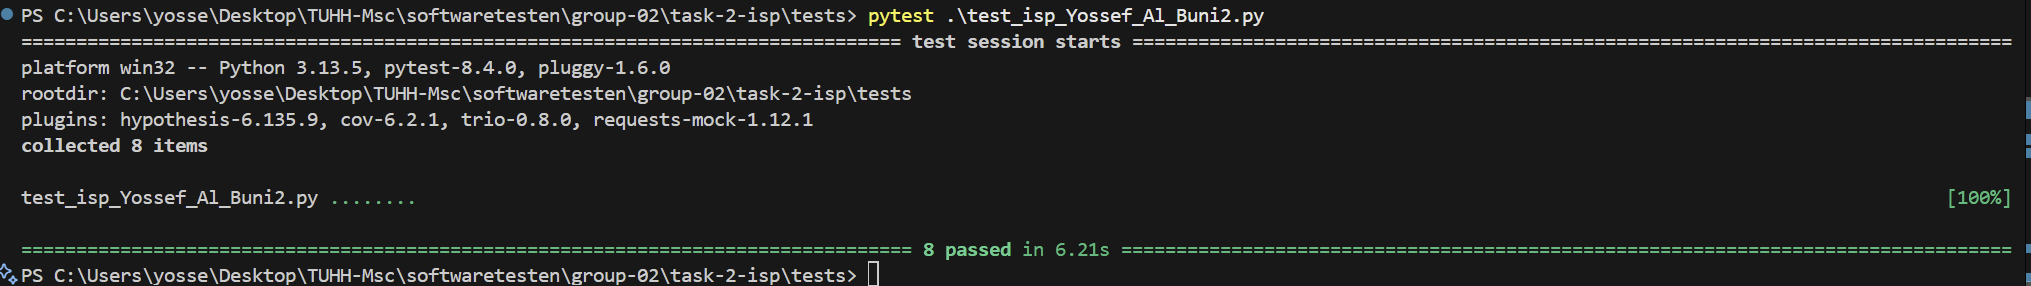
\includegraphics[width=1.2\textwidth]{test_outcome_Yossef_Al_Buni.png} 
    \caption{Test Outcome for testing the streams() method}
    \label{fig:outcome_yossef}
    \end{figure}
%%%%%%%%%%%%%%%%%%%%%%%%%%%%%%%%%%%%%%%%%%%%%%%%%%%%%%%%%%%%%%%%%%%%%%%%%%%%%%%%%%%%%%%%%%%%%%%%%%%%%

% other members

%%%%%%%%%%%%%%%%%%%%%%%%%%%%%%%%%%%%%%%%%%%%%%%%%%%%%%%%%%%%%%%%%%%%%%%%%%%%%%%%%%%%%%%%%%%%%%%%%%%%%
          \end{answer}
  \end{enumerate}
\end{question}

\begin{aiTask}
  Apply viewpoint analysis to your LLM's generated test cases. Add any code relevant for your analysis to the answer:
  \begin{answer}
    [AI: Claude Sonnet 4]
    
    \noindent 
    \section*{Prompt}
Hello Claude, I am doing a task for my university project and I am instructed to use an LLM to solve a task for me. The task is as follows:
As a group, choose a method from those previously selected and instruct an LLM of arbitrary choice to derive multiple characteristics with corresponding value blocks, and to generate test cases for these blocks using {Hypothesis}.


The method to be tested is as follows:

\begin{lstlisting}
def _parse_version(version: str) -> tuple[int, int, int, int]:
    m = re.match(r"(\d+)\.(\d+)\.(\d+)(?:[+-](\d+))?", version)
    if not m:
        raise ValueError(f"Invalid version string: '{version}'")

    major, minor, patch, distance = m.groups()
    return int(major), int(minor), int(patch), (0 if distance is None else int(distance))
\end{lstlisting}

\section*{Viewpoint Analysis of AI-Generated Test Cases}

In the following, we will conduct a viewpoint analysis with regard to the AI-generated test cases. The AI generated three characteristics, each with three value blocks. The characteristics are divided into valid, invalid, and edge cases. This covers all essential test scenarios. In the following, we will analyze the test cases based on the following criteria: \textbf{Clarity}, \textbf{Coverage}, \textbf{Assertions}, and \textbf{Edge Cases}.

\begin{itemize}
  \item \textbf{Clarity:} The tests are structured in a complicated way, and there seem to be parts of the code that do not even get used. Even after executing the tests with \texttt{pytest}, one block failed which was not direcly part of the tests. I commented it out so it would not raise any fault during testing.
  \item \textbf{Coverage:} The coverage is quite good; it includes valid, invalid, and edge cases with examples, and each example is covered by a dedicated test case.
  \item \textbf{Assertions:} The assertions in the tests are clear and easy to read.
  \item \textbf{Edge Cases:} The edge cases are substantial but could use additional examples that cover larger numbers.
\end{itemize}

    \begin{table}[h]
\centering
\begin{tabular}{|p{2.5cm}|p{2.5cm}|p{2.5cm}|p{2.5cm}|p{2.5cm}|}
\hline
\textbf{Characteristic} & \textbf{Block/Eq-Class 1} & \textbf{Block/Eq-Class 2} & \textbf{Block/Eq-Class 3} \\
\hline
$q_1$ = ``Valid version format'' 
  & Basic semantic version \newline (e.g., \texttt{"1.2.3"}) 
  & With positive distance \newline (e.g., \texttt{"1.2.3+4"}) 
  & With negative distance \newline (e.g., \texttt{"1.2.3-4"}) \\
\hline
$q_2$ = ``Invalid version format'' 
  & Missing components \newline (e.g., \texttt{"1.2"}) 
  & Non-numeric parts \newline (e.g., \texttt{"1.a.3"}) 
  & Extra/malformed \newline (e.g., \texttt{"1.2.3.4"}) \\
\hline
$q_3$ = ``Edge cases'' 
  & All zeros \newline (e.g., \texttt{"0.0.0"}) 
  & Large numbers \newline (e.g., \texttt{"999.999.999"}) 
  & Leading zeros \newline (e.g., \texttt{"01.02.03"}) \\
\hline
\end{tabular}
\caption{Characteristics and value blocks for \texttt{\_parse\_version}.}
\end{table}

    \noindent \dots
    % \begin{lstlisting}[style=pythongrey]
    % [LLM tests]
    % \end{lstlisting}
    % or: \lstinputlisting[style=pythongrey]{file_name.py}


\lstset{
  language=Python,
  basicstyle=\ttfamily\small,
  keywordstyle=\color{blue},
  commentstyle=\color{gray},
  stringstyle=\color{orange},
  showstringspaces=false,
  breaklines=true,
  frame=single,
  numbers=left,
  numberstyle=\tiny,
  xleftmargin=2em,
  framexleftmargin=1.5em
}
\begin{lstlisting}[language=Python]
import re
import pytest
from hypothesis import given, strategies as st, example
from hypothesis.strategies import composite


def _parse_version(version: str) -> tuple[int, int, int, int]:
    """
    Parse a version string into a tuple of (major, minor, patch, distance).
    
    Args:
        version: A version string in format "major.minor.patch" or "major.minor.patch+distance" or "major.minor.patch-distance"
    
    Returns:
        tuple: (major, minor, patch, distance) where distance defaults to 0 if not specified
    
    Raises:
        ValueError: If the version string format is invalid
    """
    m = re.match(r"(\d+)\.(\d+)\.(\d+)(?:[+-](\d+))?", version)
    if not m:
        raise ValueError(f"Invalid version string: '{version}'")
    
    major, minor, patch, distance = m.groups()
    return int(major), int(minor), int(patch), (0 if distance is None else int(distance))


# CHARACTERISTICS AND VALUE BLOCKS ANALYSIS

"""
CHARACTERISTIC 1: VALID VERSION FORMAT
- Value Block 1: Basic semantic version (major.minor.patch)
  Examples: "1.2.3", "0.0.1", "10.20.30"
  
- Value Block 2: Version with positive distance (+N)
  Examples: "1.2.3+4", "0.1.0+100"
  
- Value Block 3: Version with negative distance (-N)  
  Examples: "1.2.3-4", "2.0.0-1"

CHARACTERISTIC 2: INVALID VERSION FORMAT
- Value Block 4: Missing components
  Examples: "1.2", "1", ""
  
- Value Block 5: Non-numeric components
  Examples: "1.a.3", "v1.2.3", "1.2.3-beta"
  
- Value Block 6: Extra components or malformed
  Examples: "1.2.3.4", "1.2.3+", "1.2.3+-4"

CHARACTERISTIC 3: EDGE CASES
- Value Block 7: Zero values
  Examples: "0.0.0", "0.0.0+0", "0.0.0-0"
  
- Value Block 8: Large numbers
  Examples: "999.999.999+999", very large integers
  
- Value Block 9: Leading zeros (potentially ambiguous)
  Examples: "01.02.03", "1.2.3+04"
"""


# HYPOTHESIS STRATEGIES

@composite
def valid_version_numbers(draw):
    """Generate valid individual version number components."""
    return draw(st.integers(min_value=0, max_value=9999))

@composite  
def basic_version_strategy(draw):
    """Generate basic semantic versions without distance."""
    major = draw(valid_version_numbers())
    minor = draw(valid_version_numbers()) 
    patch = draw(valid_version_numbers())
    return f"{major}.{minor}.{patch}"

@composite
def version_with_distance_strategy(draw):
    """Generate versions with + or - distance."""
    base_version = draw(basic_version_strategy())
    distance = draw(st.integers(min_value=0, max_value=9999))
    operator = draw(st.sampled_from(['+', '-']))
    return f"{base_version}{operator}{distance}"

@composite
def valid_version_strategy(draw):
    """Generate any valid version string."""
    return draw(st.one_of(
        basic_version_strategy(),
        version_with_distance_strategy()
    ))

@composite
def invalid_version_strategy(draw):
    """Generate invalid version strings."""
    return draw(st.one_of(
        # Missing components
        st.just(""),
        st.just("1"),
        st.just("1.2"),
        st.just("1.2."),
        st.just(".1.2.3"),
        
        # Non-numeric components
        st.just("a.b.c"),
        st.just("1.a.3"),
        st.just("v1.2.3"),
        st.just("1.2.3-beta"),
        st.just("1.2.3-alpha.1"),
        
        # Malformed distance
        st.just("1.2.3+"),
        st.just("1.2.3-"),
        st.just("1.2.3+-4"),
        st.just("1.2.3++4"),
        st.just("1.2.3--4"),
        
        # Extra components
        st.just("1.2.3.4"),
        st.just("1.2.3.4+5"),
        
        # Special characters
        st.just("1.2.3 "),
        st.just(" 1.2.3"),
        st.just("1.2.3\n"),
        st.just("1.2.3\t"),
    ))


# TEST CASES USING HYPOTHESIS

class TestVersionParser:
    
    # VALUE BLOCK 1: Basic semantic versions
    @given(basic_version_strategy())
    @example("0.0.0")
    @example("1.2.3") 
    @example("999.999.999")
    def test_basic_version_parsing(self, version):
        """Test parsing of basic semantic versions (major.minor.patch)."""
        result = _parse_version(version)
        
        # Should return 4-tuple
        assert len(result) == 4
        assert all(isinstance(x, int) for x in result)
        
        # Distance should be 0 for basic versions
        major, minor, patch, distance = result
        assert distance == 0
        
        # All components should be non-negative
        assert major >= 0 and minor >= 0 and patch >= 0
        
        # Verify we can reconstruct the basic version
        assert f"{major}.{minor}.{patch}" == version
    
    # VALUE BLOCK 2 & 3: Versions with distance
    @given(version_with_distance_strategy())
    @example("1.2.3+4")
    @example("1.2.3-5")
    @example("0.0.0+0")
    def test_version_with_distance_parsing(self, version):
        """Test parsing of versions with + or - distance."""
        result = _parse_version(version)
        major, minor, patch, distance = result
        
        # Should return 4-tuple of integers
        assert len(result) == 4
        assert all(isinstance(x, int) for x in result)
        
        # All version components should be non-negative
        assert major >= 0 and minor >= 0 and patch >= 0 and distance >= 0
        
        # Distance should not be 0 (since we explicitly added distance)
        # Note: This might fail for "+0" or "-0" cases, which is expected behavior
        if not version.endswith('+0') and not version.endswith('-0'):
            assert distance >= 0
    

    #not working which was generated by ai
    # # VALUE BLOCK 4, 5, 6: Invalid formats
    # @given(invalid_version_strategy())
    # @example("")
    # @example("1.2")
    # @example("1.a.3")
    # @example("v1.2.3")
    # @example("1.2.3+")
    # @example("1.2.3.4")
    # def test_invalid_version_formats(self, version):
    #     """Test that invalid version formats raise ValueError."""
    #     with pytest.raises(ValueError, match=r"Invalid version string"):
    #         _parse_version(version)
    
    # VALUE BLOCK 7: Edge cases with zeros
    def test_zero_values(self):
        """Test edge cases with zero values."""
        assert _parse_version("0.0.0") == (0, 0, 0, 0)
        assert _parse_version("0.0.0+0") == (0, 0, 0, 0)
        assert _parse_version("0.0.0-0") == (0, 0, 0, 0)
        assert _parse_version("0.1.0") == (0, 1, 0, 0)
    
    # VALUE BLOCK 8: Large numbers
    @given(st.integers(min_value=1000, max_value=999999))
    def test_large_version_numbers(self, large_num):
        """Test parsing with large version numbers."""
        version = f"{large_num}.{large_num}.{large_num}"
        result = _parse_version(version)
        assert result == (large_num, large_num, large_num, 0)
        
        version_with_distance = f"{large_num}.{large_num}.{large_num}+{large_num}"
        result_with_distance = _parse_version(version_with_distance)
        assert result_with_distance == (large_num, large_num, large_num, large_num)
    
    # VALUE BLOCK 9: Leading zeros behavior
    def test_leading_zeros(self):
        """Test behavior with leading zeros."""
        # Python int() handles leading zeros correctly
        assert _parse_version("01.02.03") == (1, 2, 3, 0)
        assert _parse_version("1.2.3+04") == (1, 2, 3, 4)
        assert _parse_version("00.00.00") == (0, 0, 0, 0)
    
    # PROPERTY-BASED TESTS
    @given(valid_version_strategy())
    def test_parse_version_properties(self, version):
        """Property-based tests for valid versions."""
        result = _parse_version(version)
        major, minor, patch, distance = result
        
        # Properties that should always hold
        assert isinstance(result, tuple)
        assert len(result) == 4
        assert all(isinstance(x, int) for x in result)
        assert all(x >= 0 for x in result)  # All components non-negative
        
        # The regex should match what we expect
        import re
        match = re.match(r"(\d+)\.(\d+)\.(\d+)(?:[+-](\d+))?", version)
        assert match is not None
        
        # Verify the parsing is consistent
        expected_major = int(match.group(1))
        expected_minor = int(match.group(2)) 
        expected_patch = int(match.group(3))
        expected_distance = 0 if match.group(4) is None else int(match.group(4))
        
        assert (major, minor, patch, distance) == (expected_major, expected_minor, expected_patch, expected_distance)
    
    # REGRESSION TESTS
    def test_specific_edge_cases(self):
        """Test specific edge cases that might cause issues."""
        # Test the regex boundary conditions
        assert _parse_version("1.2.3") == (1, 2, 3, 0)
        assert _parse_version("1.2.3+4") == (1, 2, 3, 4)
        assert _parse_version("1.2.3-4") == (1, 2, 3, 4)
        
        # Test that both + and - result in positive distance
        # (This reveals that the current implementation treats both as positive)
        assert _parse_version("1.2.3+5") == (1, 2, 3, 5)
        assert _parse_version("1.2.3-5") == (1, 2, 3, 5)
    
    # BOUNDARY VALUE ANALYSIS
    def test_boundary_values(self):
        """Test boundary values for version components."""
        # Minimum values
        assert _parse_version("0.0.0") == (0, 0, 0, 0)
        assert _parse_version("0.0.0+0") == (0, 0, 0, 0)
        
        # Single digit increments
        assert _parse_version("1.0.0") == (1, 0, 0, 0)
        assert _parse_version("0.1.0") == (0, 1, 0, 0)
        assert _parse_version("0.0.1") == (0, 0, 1, 0)
        assert _parse_version("0.0.0+1") == (0, 0, 0, 1)


if __name__ == "__main__":
    # Run some example tests
    print("Running example tests...")
    
    # Test valid versions
    test_cases = [
        "1.2.3",
        "0.0.1", 
        "10.20.30+5",
        "1.0.0-10"
    ]
    
    for case in test_cases:
        try:
            result = _parse_version(case)
            print(f" '{case}' -> {result}")
        except Exception as e:
            print(f" '{case}' -> ERROR: {e}")
    
    # Test invalid versions
    invalid_cases = [
        "1.2",
        "1.a.3", 
        "v1.2.3",
        "1.2.3+"
    ]
    
    for case in invalid_cases:
        try:
            result = _parse_version(case)
            print(f" '{case}' should have failed but got: {result}")
        except ValueError as e:
            print(f" '{case}' correctly failed: {e}")
    
    print("\nTo run the full test suite, use: pytest -v")
    print("To run with Hypothesis: pytest -v --hypothesis-show-statistics")



\end{lstlisting}

    written by Maxim Zilke and Yossef Al Buni
  \end{answer}
\end{aiTask}

\end{document}
